%%%%%%%%%%%%%   END GENERAL SETTINGS  %%%%%%%%%%%%%%%%%%%%%%%

%%%%%%%%%%%%%  CAPTIONS AND OTHER PARPHERNALIA %%%%%%%%%%%%%%%%%
\cxset{steward,
  numbering=arabic,
  custom=tikzspecial,
  offsety=0cm,
  image=hine06,
  texti={A picture is worth a thousand words, but if you don't add a good description of what it is in a caption, your readers will be left scratching their heads. Here we discuss captions in general as well as the formatting commands available in LaTeX, some common packages and athena.},
%
  textii={In this chapter we discuss methods that allow the formatting and positioning of captions, based on a set of key values. Central  to this process is the separation of content from presentation.
We also discuss the basic formatting tools that are available and how one can modify them to blend them with the rest of the design.
 }
}
\chapter{Typesetting Captions}
\section{Introduction}

The formatting commands for captions follow the same style of the rest of the package.

\section{Conventions}

All caption keys start with the word caption. The float type follows, so caption figure font-size refers to the caption of a figure environment. If the figure is omitted the style is applicable both the Tables and Figures. As users will probably only set these keys only once, my recommendation is to user the longer version (it will give you finer control).
\bigskip

\keyval{caption format}{plain|hang}{ affects all captions such as tables and figures and will produce either a hang caption or with plain will wrap arund the figure number like a normal paragraph.}

\keyval{caption figure format}{\marg{plain|hang}}{Affects ONLY figure captions such as tables and figures and will produce either a hang caption or with plain will wrap around the figure number like a normal paragraph.}

\keyval{caption figure numbering style}{auto|continuous|reset on sections|custom}{}
\keyval{caption figure numbering}{arabic|alph|Alph|roman|Roman|custom}{}
\keyval{caption separator}{colon,semicolon,none,custom}{Sets the separator, such as \textbf{:} or a colon or none.}
\keyval{caption label name}{}{}
\keyval{caption before}{}{}
\keyval{caption after}{}{}


\cxset{caption format/.code=\captionsetup[figure]{format=#1}}

\cxset{caption format=hang}

\def\captionlabelfont@cx{bf}


\captionsetup[figure]{font={large,bf}}
\captionsetup[figure]{font={Large}}


\captionsetup[figure]{font=\captionlabelfont@cx}

\captionof{figure}{This is some very long text}

\section{Technical discussion}

The formatting of the caption, happens in stages like the sectioning commands.  \lstinline+\@makecaption}+  command is responsible for the typesetting and is defined in the standard LaTeX classes. The \cs{caption} and command is defined in the LaTeX kernel in the float.dtx class. As always we will start our discussion from the user command and follow it through to the typesetting macros.

When the user command \cs{caption} is processed, LaTeX checks if it is outside a float and if it is issues an error message. It then swallows the argument. It then calls \cs{@caption} which does further processing.

\begin{tcolorbox}
\begin{lstlisting}
\def\caption{%
 \ifx\@captype\@undefined
     \@latex@error{\noexpand\caption outside float}\@ehd
     \expandafter\@gobble
 \else
     \refstepcounter\@captype
     \expandafter\@firstofone
 \fi
 {\@dblarg{\@caption\@captype}}%
}
\end{lstlisting}
\end{tcolorbox}

\begin{lstlisting}
\def\caption{%
5 \ifx\@captype\@undefined
6 \@latex@error{\noexpand\caption outside float}\@ehd
7 \expandafter\@gobble
8 \else
9 \refstepcounter\@captype
10 \expandafter\@firstofone
11 \fi
12 {\@dblarg{\@caption\@captype}}%
13 }


\long\def\@caption#1[#2]#3{%
15 \par
16 \addcontentsline{\csname ext@#1\endcsname}{#1}%
17 {\protect\numberline{\csname the#1\endcsname}{\ignorespaces #2}}%
18 \begingroup
        \@parboxrestore
20 \if@minipage
21     \@setminipage
22 \fi
23 \normalsize
24 \@makecaption{\csname fnum@#1\endcsname}{\ignorespaces #3}\par
25 \endgroup}
\end{lstlisting}



\begin{tcolorbox}
\begin{lstlisting}
\newlength\abovecaptionskip
\newlength\belowcaptionskip
\setlength\abovecaptionskip{10\p@}
\setlength\belowcaptionskip{0\p@}

\long\def\@makecaption#1#2{%
  \vskip\abovecaptionskip
  \sbox\@tempboxa{#1: #2}
  \ifdim \wd\@tempboxa >\hsize
    #1: #2\par
  \else
    \global \@minipagefalse
    \hb@xt@\hsize{\hfil\box\@tempboxa\hfil}%
  \fi
  \vskip\belowcaptionskip}

\newcommand\listoffigures{%
    \if@twocolumn
      \@restonecoltrue\onecolumn
    \else
      \@restonecolfalse
    \fi
    \chapter*{\listfigurename}%
      \@mkboth{\MakeUppercase\listfigurename}%
              {\MakeUppercase\listfigurename}%
    \@starttoc{lof}%
    \if@restonecol\twocolumn\fi
    }
\end{lstlisting}
\end{tcolorbox}

\clearpage

In the athena package this is set as a property via a key-value interface and hence we can use a normal chapter. If it need be we can define a special chapter style only for this heading. This way we can control all aspects of the formatting of the head.

The List of Figures for example in many Social Sciences books is typed as List of Illustrations and also adds credits.


\begin{figure}[htp]
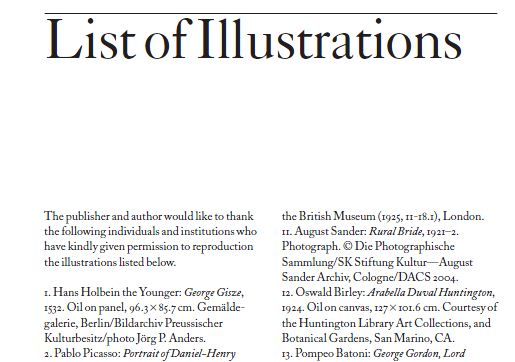
\includegraphics[width=\textwidth]{listofillustrations}
\caption{List of Illustrations extract from \textit{Oxford History of Art, Portraiture}, Shearer West, Oxford University Press, 2004.}
\end{figure}
\begin{figure}[htp]
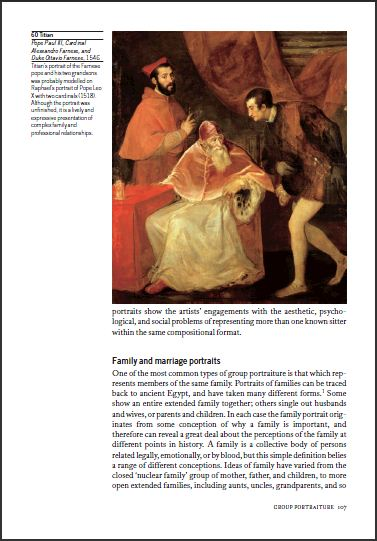
\includegraphics[width=0.67\textwidth]{titian}
\centering
\caption{Figure from \textit{Oxford History of Art, Portraiture}, Shearer West, Oxford University Press, 2004. The figures are numbered consecutively and the text in the List of Illustrations have different formatting.}
\end{figure}

\section{Formatting the List of Figures Heading}

LaTeX formats the list of figures heading in a similar manner to that of the Table of Contents. The Title `List of Figures` is obtained from the \cs{listfigurename} and which is also accessible from Babel. It does not add an entry to the ToC.



It’s good to know that \cs{captionsetup} has an effect on the current environment only.
So if you want to change settings for the current figure or table only, just place the
\cs{captionsetup} command inside the figure or table right before the \cs{caption}
command.


Many of the caption figures can be changed within LaTeX itself. For example to get continuous numbering in the book class.

\begin{lstlisting}
\makeatletter
\@removefromreset{table}{chapter}
\renewcommand{\thetable}{\arabic{table}}
\makeatother
\end{lstlisting}

The command \cs{removefromreset} can be found by loading the remreset package. Other combinations are also possible.

\keyval{caption numbering scheme}{default|continuous|chapter|section....}{The numbering style either continous or reset per spacing etc...}

\begin{marglist}
\item{continuous} Typesets numbers from 1 to ...... without any resetting
\end{marglist}
% Date: Sat, 30 Jul 1994 17:58:55 PST
% From: Donald Arseneau <asnd@erich.triumf.ca>
%
%  \@removefromreset{FOO}{BAR} : Removes counter FOO from the list of
%                       counters \cl@BAR to be reset when counter BAR
%                       is stepped.  The opposite of \@addtoreset.

\def\@removefromreset#1#2{\let\@tempb\@elt
   \expandafter\let\expandafter\@tempa\csname c@#1\endcsname
   \def\@elt##1{\expandafter\ifx\csname c@##1\endcsname\@tempa\else
         \noexpand\@elt{##1}\fi}%
   \expandafter\edef\csname cl@#2\endcsname{\csname cl@#2\endcsname}%
   \let\@elt\@tempb}

\@removefromreset{figure}{chapter}
\renewcommand{\thefigure}{\arabic{figure}}

\@specialfalse\@tocfalse
% need additional boolean in toc
\begin{texexample}{}{}
\setdefaults
\cxset{chapter opening=anywhere,
          chapter font-size=\normalfont,
          title font-size=\large}


\gdef\continuousfigures@cx{\@removefromreset{figure}{chapter}
\gdef{\thefigure}{\arabic{figure}}}

\cxset{caption numbering continuous/.code={\continuousfigures@cx}}


\chapter{This is the First Chapter}
\captionof{figure}{test}
\captionof{figure}{test}
\chapter{This is the Second Chapter}
\captionof{figure}{test}
\captionof{figure}{test}
\end{texexample}


\begin{figure}[htp]
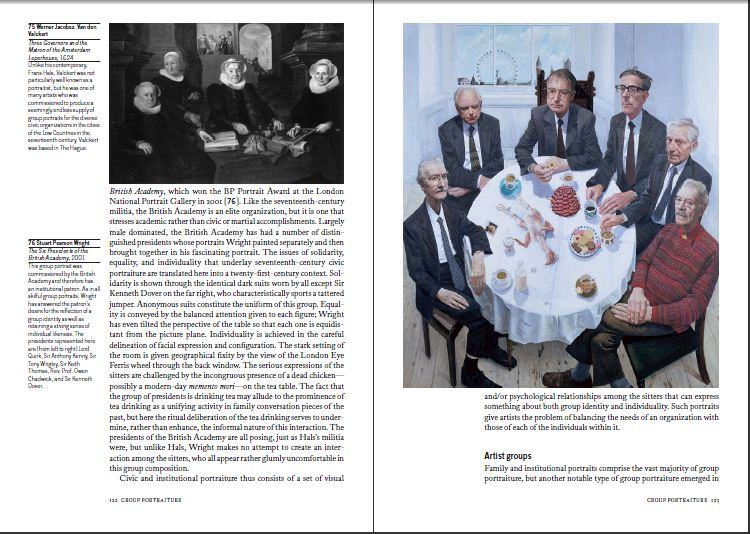
\includegraphics[width=0.98\textwidth]{captionspecial}
\centering
\caption{Figure from \textit{Oxford History of Art, Portraiture}, Shearer West, Oxford University Press, 2004. The figures are numbered consecutively and the text in the List of Illustrations have different formatting.}
\end{figure}


% Note with new geometry paper has to be defined in preamble
% I do not feel very confident of this
% Don't understand it fully how is working

\cxset{geometry oxford/.code={
\newgeometry{a4paper,left=74.8mm,top=27.4mm,headsep=2\baselineskip,%
marginparsep=8.2mm,marginparwidth=49.4mm,textheight=49\baselineskip,headheight=\baselineskip}
\@twosidefalse \@mparswitchfalse % one side option
\reversemarginpar
}}

\cxset{geometry textwidth/.store in=\textwidth@cx,
          geometry textheight/.store in=\textheight@cx,
          geometry tufte/.code={
             \newgeometry{a4paper,left=24.8mm,top=27.4mm,headsep=2\baselineskip,%
             textwidth=107mm,marginparsep=8.2mm,marginparwidth=49.4mm,%
             textheight=\textheight@cx\baselineskip,headheight=\baselineskip}
            \@twosidefalse \@mparswitchfalse % one side option
           %\reversemarginpar
    }
}

\cxset{marginpar push/.store in=\marginparpush@cx,
          marginpar font/.store in=\marginparfont@cx,
          marginpar justification/.is choice,
          marginpar justification/justifying/.code=\gdef\marginparjustification@cx{\justifying},
          marginpar justification/raggedright/.code=\gdef\marginparjustification@cx{\raggedright},
          marginpar justification/RaggedRight/.code=\gdef\marginparjustification@cx{\RaggedRight},
          marginpar justification/RaggedLeft/.code=\gdef\marginparjustification@cx{\RaggedLeft},
 }
\cxset{marginpar push=10pt,
          marginpar font=\normalfont\footnotesize\sffamily,
          marginpar justification=RaggedLeft}

\cxset{style13, geometry textheight=49,
          geometry oxford,
          watermark text=SAMPLE TUFTE VARIANT,
          watermark text color=thered,
          header style=samplepage}

% This is a sidenote without the footnote mark
\newcommand\marginnote[2][0pt]{%
 % \let\cite\@tufte@infootnote@cite%   use the in-sidenote \cite command
  %\gdef\@tufte@citations{}%           clear out any old citations
  \@tufte@margin@par%                 use parindent and parskip settings for marginal text
  \marginpar{\hbox{}\vspace*{#1}\marginparfont@cx\marginparjustification@cx\vspace*{-1\baselineskip}\noindent #2}%
  \@tufte@reset@par%                  use parindent and parskip settings for body text
  %\@tufte@print@citations%            print any citations
  %\let\cite\@tufte@normal@cite%       go back to using normal in-text \cite command
}

\chapter{Geometry and Page Dimensions}

\lipsum[1-4]\marginnote[1pt]{\lorem
    \lorem}

\lipsum[1-2]

%% Stick the caption in the head might as well place the first picture also
\def\asidecaption{\parbox{4.2cm}{{\bfseries Image \thefigure}\par\lorem}%
  % \addtocontents{lof}{This is image 8}
}
\def\ps@caption{%
     \let\@oddfoot\@empty\let\@evenfoot\@empty%
    \def\@evenhead{%
        \begin{picture}(0,0)%
           \put(-150,-80){\asidecaption\par}%
            \stepcounter{figure}
           \put(-150,-370){\asidecaption}%
        \end{picture}%
      }%
    \let\@oddhead\@evenhead%
    \let\@mkboth\@gobbletwo%
    \let\chaptermark\@gobble%
    \let\sectionmark\@gobble%
 }

\def\ps@bigpicture{%
    \setlength\headheight{19cm}%
    \let\@oddfoot\@empty\let\@evenfoot\@empty%
    \def\@evenhead{%
         \begin{picture}(0,0)%
          \put(-149,0){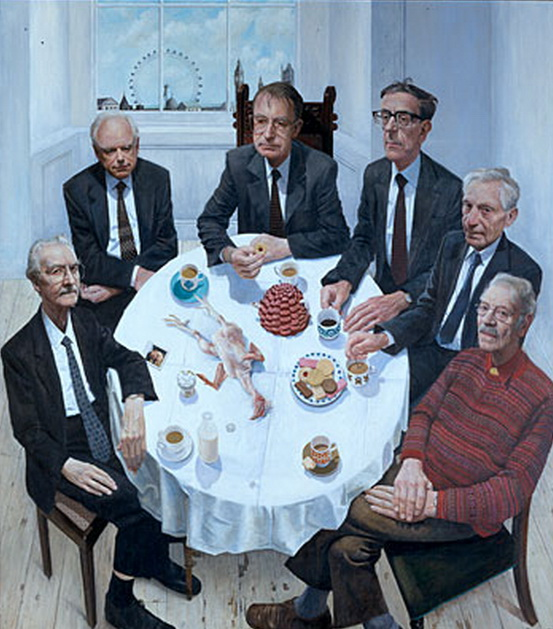
\includegraphics[width=\dimexpr(\textwidth+150pt)]{stuartpearson}}%
         \end{picture}%
      }%
    \let\@oddhead\@evenhead%
    \let\@mkboth\@gobbletwo%
    \let\chaptermark\@gobble%
    \let\sectionmark\@gobble%
 }


\def\doubletakeimage{%
  \renewcommand{\topfraction}{.95}  % ensure seecond image will not float away
  \begin{figure}[t]
    \thispagestyle{caption}
    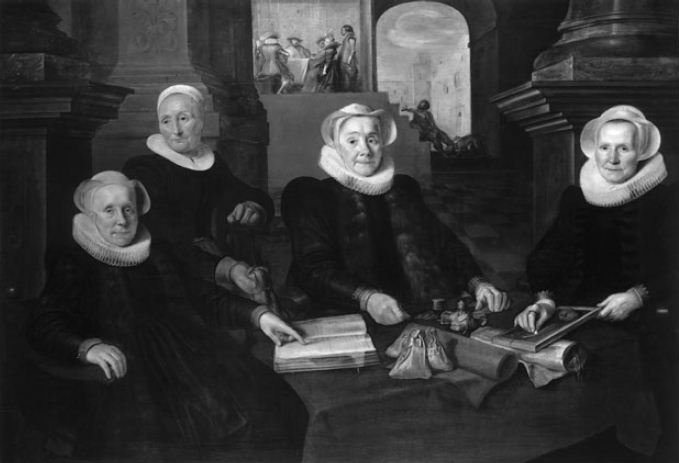
\includegraphics[width=\textwidth]{matron}%
  \end{figure}

  \begin{figure}[tp]
   \hspace*{-\marginparwidth}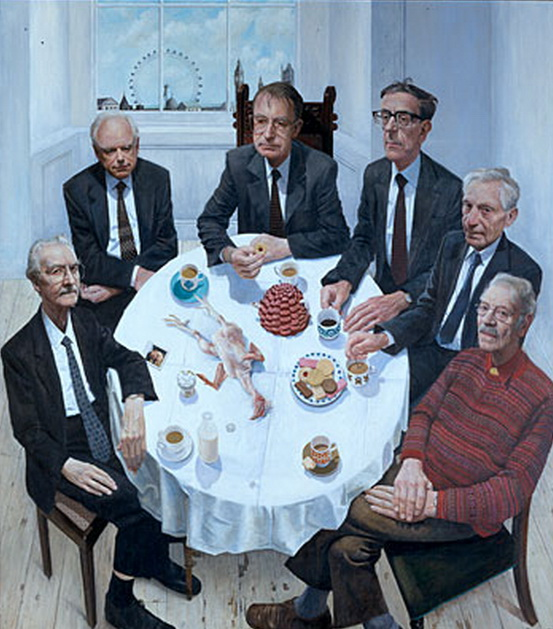
\includegraphics[height=0.9\textheight]{stuartpearson}
 \end{figure}
}


\doubletakeimage
\lipsum[1-4]

\restoregeometry
%% RESET EVERYTHING AT END OF CHAPTER
\addtocounter{chapter}{-2}
\@toctrue\@specialtrue

